\documentclass{article}

\usepackage[a4paper, total={6in, 8in}]{geometry}

\usepackage{amsmath}
\usepackage{amsfonts}
\usepackage{amssymb}
\usepackage[T1, T2A]{fontenc}
\usepackage[utf8]{inputenc}
\usepackage[english, russian]{babel}
\usepackage{graphics}
\usepackage{graphicx}
\usepackage{multicol}
\usepackage{mwe}

\geometry{
 a4paper,
 total={170mm,257mm},
 left=20mm,
 top=20mm,
 }

\author{Александр Валентинов}
\title{Лабораторная работа 3.2.4}

\begin{document}
   \subsection*{Работа 3.2.1}
   \section*{Сдвиг фаз в цепи переменного тока.}
   
   \paragraph{Цель работы} изучить влияние активного сопротивления, индуктивности и емкости на сдвиг фаз между током и напряжением в цепи переменного тока.
   
   \paragraph{В работе используются:} генератор звуковой частоты, двузканальной осциллограф, магазин емкостей, магазин соаротивлений катушка индуктивности, резисторы, мост переменного тока.

   \subsubsection*{Теория}
   Циклическая частота: \[ \Omega = 2\pi\nu. \]
   Реактивное сопротивление емкости: \[ Z = \frac{1}{\Omega C}. \]
   Реактивное сопротивление индуктивности: \[ Z = \Omega L. \]
   Сдвиг фаз между синусоидами на двухканальном осциллографе: 
   \begin{equation}
   \label{psi} 
   \psi = \pi \cdot \frac{x}{x_0},~~~ \sigma_\psi = \pi\sqrt{\left( \frac{\sigma_x}{x_0} \right)^2 + \left( \frac{x}{x_0} \frac{\sigma_{x_0}}{x_0} \right)^2};
   \end{equation}
   где $x$ --- расстояния между нулевыми значениями синусоид, $x_0$ --- расстояния между нулевыми значениями одного из сигналов. 

   \subsubsection*{Экспериментальная установка:}   
  % \begin{figure}[h!]
  %     \centering
  %     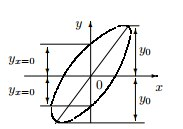
\includegraphics[height=.2\textwidth]{fig1.jpg}
  %     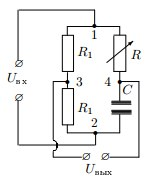
\includegraphics[height=.2\textwidth]{fig2.jpg}
  %     \caption{Блабла}
  % \end{figure}

   \begin{figure}[h]
   \centering
   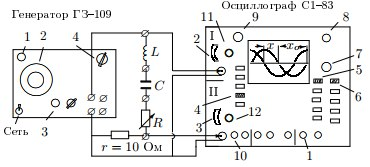
\includegraphics[width=8cm]{fig3.jpg} 
   \caption{Схема установки для исследования сдвига фаз между током и напряжением.} 
   \label{fig.1} 
   \end{figure}

   \begin{figure}[h]
   \centering
   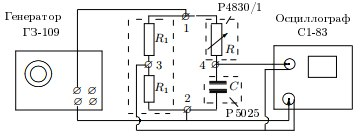
\includegraphics[width=8cm]{fig4.jpg} 
   \caption{Схема установки для исследования фазовращателя.} 
   \label{fig.4} 
   \end{figure}
   
   \subsubsection*{Обработка результатов}
   \subparagraph*{RC-цепь.}
   Построим график $\tan \psi = f[1 / (\Omega C R_{\Sigma})] \equiv f(X)$, где $R_\Sigma = R + r$. Теоретический график будет иметь коэффициент наклона 1 и пересечение с осью $\tan \psi$ в точке $0$. Рассчитаем $\psi$ по формуле \eqref{psi}. Результаты в таблице \ref{RCtable} и на рисунке \ref{plot1}.

   \begin{table} 
 \caption{Зависимость для RC-цепи}
 \label{RCtable}
\begin{center}
\begin{tabular}{|*{4}{r|}}
\hline 
$\psi$ & $\tan \psi$ & $\sigma_{\tan_\psi}$ & $1 / (\Omega C R_\Sigma)$ \\ \hline 
 1.51 & 16   & 1    & 25.7  \\ \hline 
 1.26 & 3.1  & 0.2  & 2.83  \\ \hline 
 1.01 & 1.6  & 0.1  & 1.65  \\ \hline 
 0.75 & 0.94 & 0.09 & 0.93  \\ \hline 
 0.50 & 0.55 & 0.07 & 0.566 \\ \hline 
 0.25 & 0.26 & 0.07 & 0.260 \\ \hline 
 0.00 & 0.00 & 0.06 & 0.099 \\ \hline 
 \end{tabular}
\end{center} 
\end{table} 

   \begin{figure}[h]
   \centering
   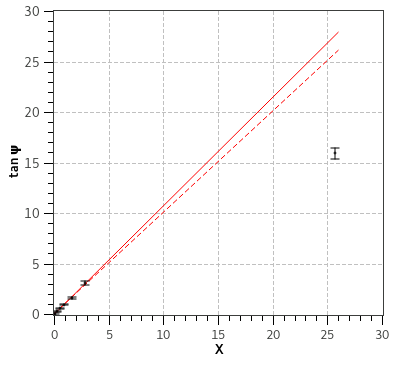
\includegraphics[width=8cm]{plot1.png} 
   \caption{Зависимость $\tan \psi (X)$} 
   \label{plot1} 
   \end{figure}

   Коэффициент наклона графика: $1.03 \pm 0.04$, что сходится с теорией.

   \subparagraph*{RL-цепь.}
   Построим график $\tan \psi = f[\Omega L / R_{\Sigma}] \equiv f(Y)$, где $R_\Sigma = R + r + R_L$. Теоретический график будет иметь коэффициент наклона 1 и пересечение с осью $\tan \psi$ в точке $0$. Рассчитаем $\psi$ по формуле \eqref{psi}. Результаты в таблице \ref{RLtable} и на рисунке \ref{plot2}.

   \begin{table} 
 \caption{Table2}
\begin{tabular}{|*{8}{c|}}
\hline 
I & Ex0.3 & Ex0.45 & Ex0.5 & Ex0.65 & Ex0.8 & Ex0.95 & Ex-0.95\\ \hline 
17.2 & 0 & 0 & 0 & 0 & 0 & 0 & 0 \\ \hline 
 181.9 & 0.051 & 0.072 & 0.084 & 0.109 & 0.129 & 0.159 & 0.166 \\ \hline 
 378.1 & 0.103 & 0.151 & 0.169 & 0.218 & 0.266 & 0.319 & 0.328 \\ \hline 
 571.8 & 0.151 & 0.224 & 0.251 & 0.322 & 0.396 & 0.472 & 0.496 \\ \hline 
 730.7 & 0.195 & 0.288 & 0.323 & 0.417 & 0.508 & 0.605 & 0.64 \\ \hline 
 854.4 & 0.228 & 0.336 & 0.378 & 0.487 & 0.595 & 0.71 & 0.75 \\ \hline 
 934.9 & 0.251 & 0.368 & 0.418 & 0.535 & 0.655 & 0.781 & 0.831 \\ \hline 
 1,003 & 0.269 & 0.394 & 0.446 & 0.569 & 0.698 & 0.83 & 0.884 \\ \hline 
 \end{tabular} 
\end{table} 

   \begin{figure}[h]
   \centering
   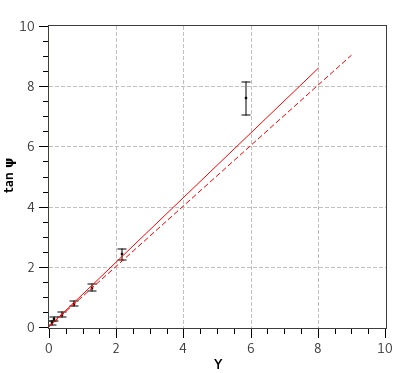
\includegraphics[width=8cm]{plot2.png} 
   \caption{Зависимость $\tan \psi (X)$} 
   \label{plot2} 
   \end{figure}
   Коэффициент наклона графика: $1.04 \pm 0.05$, что сходится с теорией.

   \subparagraph*{RLC-цепь.}
   Построим графики $| \psi | = f(\nu / \nu_0)$ для $R = 0$ и $R = 100$. Выберем масштаб оси $\psi$ $\pi / 16$. Результаты в таблицах \ref{RLCtable1}, \ref{RLCtable2} и на рисунке \ref{plot3}.

   \begin{table} 
 \caption{Table3}
\begin{tabular}{|*{3}{c|}}
\hline 
f & delta nu & 1\\ \hline 
1 & 1.0 & 0.1 \\ \hline 
 2 & 2.0 & 0.2 \\ \hline 
 3 & 2.5 & 0.1 \\ \hline 
 4 & 5.0 & 0.5 \\ \hline 
 5 & 5.0 & 0.6 \\ \hline 
 6 & 5.7 & 0.5 \\ \hline 
 7 & 6.7 & 0.7 \\ \hline 
 8 & 7.5 & 0.8 \\ \hline 
 \end{tabular} 
\end{table} 

   \begin{table}
\caption{Зависимость для RLC-контура при $R = 100$ Ом}
 \label{RLCtable2}
 \begin{center}
\begin{tabular}{|*{4}{r|}}
\hline 
$\nu$, Гц & $\psi$ & $\sigma_\psi$ & $\nu / \nu_0$ \\ \hline  
700 & 0.99 & 0.05 & 0.70 \\ \hline 
 760 & 0.88 & 0.05 & 0.76 \\ \hline 
 810 & 0.73 & 0.05 & 0.81 \\ \hline 
 870 & 0.58 & 0.06 & 0.87 \\ \hline 
 910 & 0.35 & 0.06 & 0.91 \\ \hline 
 980 & 0.13 & 0.06 & 0.98 \\ \hline 
 1,000 & 0.00 & 0.07 & 1.00 \\ \hline 
 1,020 & 0.13 & 0.07 & 1.02 \\ \hline 
 1,100 & 0.41 & 0.07 & 1.10 \\ \hline 
 1,240 & 0.79 & 0.08 & 1.24 \\ \hline 
 1,500 & 1.05 & 0.11 & 1.50 \\ \hline 
 \end{tabular} 
 \end{center}
\end{table}
   \begin{figure}[h]
   \centering
   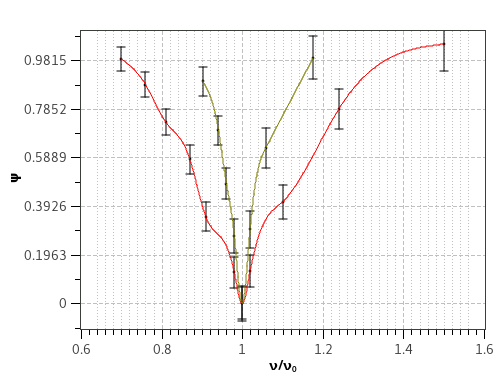
\includegraphics[width=8cm]{plot3.png} 
   \caption{Зависимость $| \psi | = f(\nu / \nu_0)$} 
   \label{plot3} 
   \end{figure} 

   Рассчитаем добротности по графикам:
   \[
     Q_{R = 0} = 1/(1.10 - 0.92) = 5.56,~~~ Q_{R = 100} = 1/(1.24 - 0.78) = 2.17
   \]
   Рассчитаем добротности по формуле
   \[
     Q = \frac{1}{R}\sqrt{\frac{L}{C}}
   \]~\[
     Q_{R = 0}^{\text{теор}} = 9.56,~~~ Q_{R = 100}^{\text{теор}} = 2.37
   \]
   Теоретические значения больше полученных экспериментально, т.к. они не учитывают сопротивление соединительных проводов, а также эффекты, возникающие в катушке и конденсаторе.

   \begin{figure}[h]
   \centering
   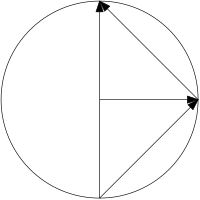
\includegraphics[width=4cm]{fig5.png} 
   \caption{Векторная диаграмма фазовращателя} 
   \label{fig1} 
   \end{figure} 
\end{document}
